%%%%%%%%%%%%%%%%%%%%%%%%%%%%%%%%%%%%%%%%%%%%%%%%%%%%%%%%%%%%%%%%%%%%%
% LaTeX Template: Project Titlepage Modified (v 0.1) by rcx
%
% Original Source: http://www.howtotex.com
% Date: February 2014
% 
% This is a title page template which be used for articles & reports.
% 
% This is the modified version of the original Latex template from
% aforementioned website.
% 
%%%%%%%%%%%%%%%%%%%%%%%%%%%%%%%%%%%%%%%%%%%%%%%%%%%%%%%%%%%%%%%%%%%%%%

\documentclass[12pt]{article}
\usepackage[a4paper]{geometry}
\usepackage[myheadings]{fullpage}
\usepackage{fancyhdr}
\usepackage{lastpage}
\usepackage{graphicx, wrapfig, subcaption, setspace, booktabs}
\usepackage[utf8]{inputenc}
\usepackage[T1]{fontenc}
\usepackage[font=small, labelfont=bf]{caption}
\usepackage{fourier}
\usepackage[protrusion=true, expansion=true]{microtype}
\usepackage[french]{babel}
\usepackage{caption}
\usepackage{sectsty}
\usepackage{url, lipsum}
\usepackage{amsmath}
\usepackage{amssymb}
\usepackage{enumerate}



\usepackage{tikz}
\usepackage[most]{tcolorbox}
\usepackage[pstricks]{bclogo}
\usepackage{pst-blur}




\newcommand{\HRule}[1]{\rule{\linewidth}{#1}}
\onehalfspacing
\setcounter{tocdepth}{5}
\setcounter{secnumdepth}{5}

%-------------------------------------------------------------------------------
% HEADER & FOOTER
%-------------------------------------------------------------------------------
\pagestyle{fancy}
\fancyhf{}
\setlength\headheight{15pt}
\fancyhead[L]{BTS CPRP 1}
\fancyhead[R]{Lycée Le Corbusier}
\fancyfoot[R]{Page \thepage\ sur \pageref{LastPage}}
\fancyfoot[L]{TP - Industrialisation}
%-------------------------------------------------------------------------------
% TITLE PAGE
%-------------------------------------------------------------------------------
 
 

%%%%POUR FAIRE DES EXERCICES INDÉPENDAMMENT DES SECTIONS%%%%
%%%%%%%%%%%%%%%%%%%%%%%%%%%%%%%%%%%%%%%%%%%%%%%%%%%%%%%%%%%%%%%%%%%
\newcounter{exo}
\newenvironment{exo}{\stepcounter{exo}\vspace{0.5cm}{\bfseries Question \theexo\ :}}{\par\vspace{0.5cm}}
%%%%%%%%%%%%%%%%%%%%%%%%%%%%%%%%%%%%%%%%%%%%%%%%%%%%%%%%%%%%%%%%%%%%




\begin{document}
 
\title{ 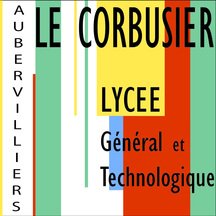
\includegraphics[width=0.18\linewidth]{Images/corbu.jpg} \hspace{2cm} \normalsize \textsc{TP Industrialisation noté \hspace{2cm} 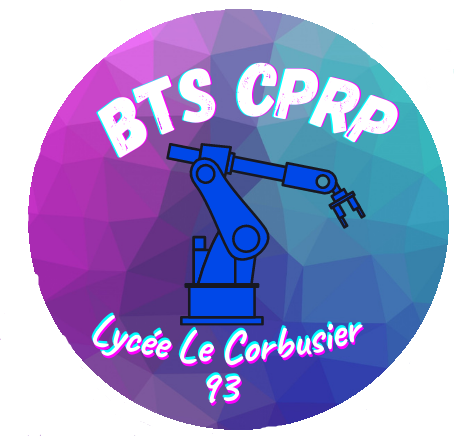
\includegraphics[width=0.2\linewidth]{Images/logo.png}}
		\\ [2.0cm]
		\HRule{0.5pt} DOSSIER SUJET \\
		\LARGE \textbf{\uppercase{TP2.1 Désignation des outils de production}}
		\HRule{2pt} \\ [0.5cm]}
\maketitle

\textbf{Deux personnes par groupe}\\
\begin{center}
Toutes les questions seront traitées dans le document réponse fourni
\end{center}










%-------------------------------------------------------------------------------
% Section title formatting
\sectionfont{\scshape}




\newpage



%%%%%%%%%%%%%%%%%%%%%%%%%%%%%%%%%%%%%%%%%%%%%%%%%%%%%%%%%%%%%%%%
%%%%%%%%%%%%%%%% MACHINE 1 %%%%%%%%%%%%%%%%%%%%%%%%%%%%%%%%%%%%%
%%%%%%%%%%%%%%%%%%%%%%%%%%%%%%%%%%%%%%%%%%%%%%%%%%%%%%%%%%%%%%%%

\tableofcontents
\newpage



\section{Conseils pour le TP}
  \bcinfo Comme pour tous les TPs, il est conseillé de lire toutes les pages une première fois, comme pour un sujet de BTS. Vous noterez que beaucoup d'informations se trouvent dans les annexes (comme au BTS). Certaines définitions et figures sont "en plus". Avant de poser une question, lisez bien tout le dossier. Ne perdez pas de temps, car les TPs sont conçus pour la durée entière : 3h. En plus de comprendre et apprendre, vous devrez écrire vos réponses au propre. Il vous est fortement conseillé de vous partager le travail entre vous deux. Vous ne devez cependant pas communiquer avec d'autres groupes.

\subsection{Matériel}

Crayon, crayons de couleur, stylos, règle et vos cours sont autorisés.

\subsection{Notation}
\noindent
Propreté et clarté dans les réponses : $\pm$3 points\\
Ne répondre que sur le document réponse.\\


\section{Objectifs :}
\begin{center}
\textbf{Découvrir les différents outils nécessaires à la production.}\\
\end{center}

\begin{minipage}[t]{.55\linewidth}
\textit{Compétences transversales travaillées :}
\begin{itemize}
    \item C11 : Définir et mettre en œuvre des essais réels et simulés
\end{itemize}

\end{minipage}
\begin{minipage}[t]{.44\linewidth}
\textit{Savoirs du programme travaillées :}
\begin{itemize}
    \item S5.3 – Conception des outils et porte-outils;
    \item S5.3.3 – Outils;
    \item S7.2.2 – Enlèvement de matière par cisaillement;
    \item S8.1.1 – Élaboration d’avant-projets (outillages retenus);
    \item S8.2 – Paramètres de génération des entités.
\end{itemize}
\end{minipage}

\section{Introduction générale}
\subsection{Process de planification de la production}
%%%%%%%%%%%%%%%%%%%%%%%%%%%%%%%%%%%%%%%%%%%%%%%%%%%%%%%%%%%%%%%%%%
%%%%%%%%%%%%%%%%%%%%%%%%%%%%%%%%%%%%%%%%%%%%%%%%%%%%%%%%%%%%%%%%
\begin{figure}[h]
\centering
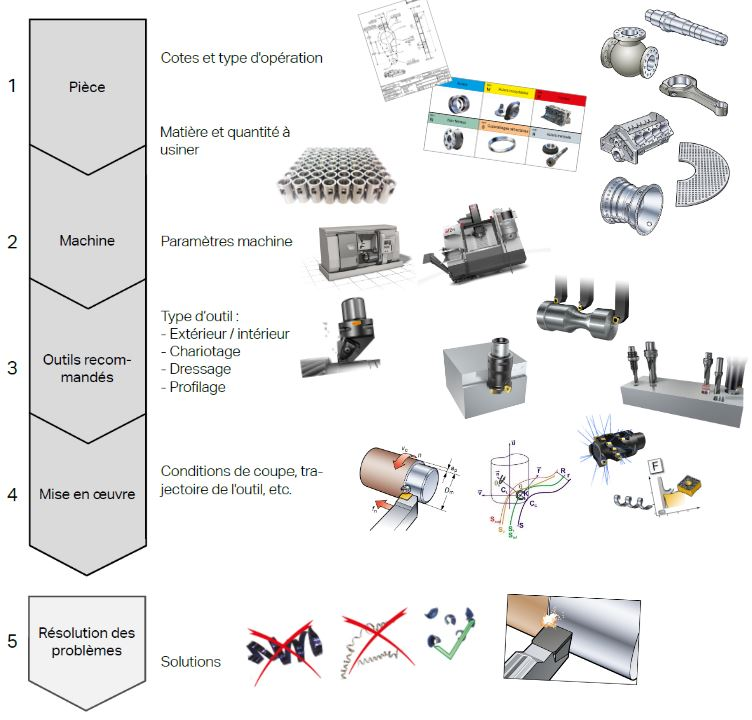
\includegraphics[width=0.93\linewidth]{Images/P1.JPG}
\caption{Au cours du BTS CPRP option sérielle, nous découvrirons toutes les étapes des processus pour réaliser une pièce voulue. Ce TP s'insère dans la $3^{ème}$ étape de la figure ci-dessus.}
\label{P1}
\end{figure}
%%%%%%%%%%%%%%%%%%%%%%%%%%%%%%%%%%%%%%%%%%%%%%%%%%%%%%%%%%%%%%%%%%
%%%%%%%%%%%%%%%%%%%%%%%%%%%%%%%%%%%%%%%%%%%%%%%%%%%%%%%%%%%%%%%%%%%


\newpage

\begin{center}



\tikzset{every picture/.style={line width=0.75pt}} %set default line width to 0.75pt        

\begin{tikzpicture}[x=0.75pt,y=0.75pt,yscale=-1,xscale=1]
%uncomment if require: \path (0,300); %set diagram left start at 0, and has height of 300

%Shape: Cube [id:dp3106942406783879] 
\draw   (163,100) -- (183,80) -- (244.55,80) -- (244.55,138) -- (224.55,158) -- (163,158) -- cycle ; \draw   (244.55,80) -- (224.55,100) -- (163,100) ; \draw   (224.55,100) -- (224.55,158) ;
%Shape: Cube [id:dp28620513900019806] 
\draw   (167,190) -- (175,182) -- (236,182) -- (236,240) -- (228,248) -- (167,248) -- cycle ; \draw   (236,182) -- (228,190) -- (167,190) ; \draw   (228,190) -- (228,248) ;
%Shape: Donut [id:dp532385415757469] 
\draw   (186,218) .. controls (186.71,211.92) and (192.22,207) .. (198.29,207) .. controls (204.37,207) and (208.71,211.92) .. (208,218) .. controls (207.29,224.08) and (201.78,229) .. (195.71,229) .. controls (189.63,229) and (185.29,224.08) .. (186,218)(180,218) .. controls (181.1,208.61) and (189.61,201) .. (199,201) .. controls (208.39,201) and (215.1,208.61) .. (214,218) .. controls (212.9,227.39) and (204.39,235) .. (195,235) .. controls (185.61,235) and (178.9,227.39) .. (180,218) ;

%Straight Lines [id:da30920672663549875] 
\draw    (506,50) .. controls (506.5,52.31) and (505.6,53.71) .. (503.29,54.2) .. controls (500.98,54.69) and (500.08,56.09) .. (500.57,58.4) .. controls (501.07,60.71) and (500.17,62.11) .. (497.86,62.6) .. controls (495.55,63.09) and (494.65,64.49) .. (495.15,66.8) .. controls (495.64,69.11) and (494.74,70.51) .. (492.43,71) .. controls (490.12,71.49) and (489.22,72.89) .. (489.72,75.2) .. controls (490.21,77.51) and (489.31,78.91) .. (487,79.4) .. controls (484.69,79.89) and (483.79,81.29) .. (484.29,83.6) .. controls (484.79,85.91) and (483.89,87.31) .. (481.58,87.8) .. controls (479.27,88.29) and (478.37,89.69) .. (478.86,92) .. controls (479.36,94.31) and (478.46,95.71) .. (476.15,96.2) .. controls (473.84,96.69) and (472.94,98.09) .. (473.44,100.4) .. controls (473.93,102.71) and (473.03,104.1) .. (470.72,104.59) -- (469.97,105.76) -- (465.63,112.48) ;
\draw [shift={(464,115)}, rotate = 302.87] [fill={rgb, 255:red, 0; green, 0; blue, 0 }  ][line width=0.08]  [draw opacity=0] (8.93,-4.29) -- (0,0) -- (8.93,4.29) -- cycle    ;
%Straight Lines [id:da36333605403726166] 
\draw    (506,50) .. controls (508.34,49.7) and (509.66,50.72) .. (509.95,53.06) .. controls (510.25,55.4) and (511.57,56.42) .. (513.91,56.12) .. controls (516.25,55.82) and (517.57,56.84) .. (517.86,59.18) .. controls (518.15,61.52) and (519.47,62.54) .. (521.81,62.24) .. controls (524.15,61.94) and (525.47,62.96) .. (525.77,65.3) .. controls (526.06,67.64) and (527.38,68.66) .. (529.72,68.37) .. controls (532.06,68.07) and (533.38,69.09) .. (533.68,71.43) .. controls (533.97,73.77) and (535.29,74.79) .. (537.63,74.49) .. controls (539.97,74.19) and (541.29,75.21) .. (541.58,77.55) .. controls (541.88,79.89) and (543.2,80.91) .. (545.54,80.61) .. controls (547.88,80.31) and (549.2,81.33) .. (549.49,83.67) .. controls (549.78,86.01) and (551.1,87.03) .. (553.44,86.73) .. controls (555.78,86.43) and (557.1,87.45) .. (557.4,89.79) .. controls (557.69,92.13) and (559.01,93.15) .. (561.35,92.85) .. controls (563.69,92.55) and (565.01,93.57) .. (565.3,95.91) .. controls (565.6,98.25) and (566.92,99.27) .. (569.26,98.97) .. controls (571.6,98.67) and (572.92,99.69) .. (573.21,102.03) -- (574.8,103.27) -- (581.13,108.16) ;
\draw [shift={(583.5,110)}, rotate = 217.75] [fill={rgb, 255:red, 0; green, 0; blue, 0 }  ][line width=0.08]  [draw opacity=0] (8.93,-4.29) -- (0,0) -- (8.93,4.29) -- cycle    ;
%Curve Lines [id:da7549614981673118] 
\draw    (282,115) .. controls (284.23,113.65) and (285.92,114.04) .. (287.09,116.19) .. controls (287.72,118.4) and (289.11,119.24) .. (291.26,118.71) .. controls (293.63,118.58) and (294.82,119.72) .. (294.82,122.15) .. controls (294.57,124.52) and (295.57,125.87) .. (297.81,126.2) .. controls (300.1,126.81) and (300.91,128.27) .. (300.24,130.58) .. controls (299.43,132.83) and (300.08,134.33) .. (302.17,135.08) .. controls (304.37,136.31) and (304.91,137.94) .. (303.79,139.97) .. controls (302.59,141.93) and (302.99,143.51) .. (304.98,144.72) .. controls (306.94,146.07) and (307.23,147.73) .. (305.86,149.7) .. controls (304.42,151.6) and (304.61,153.33) .. (306.43,154.89) .. controls (308.18,156.22) and (308.26,157.82) .. (306.66,159.69) .. controls (304.99,161.48) and (304.97,163.11) .. (306.6,164.59) .. controls (308.15,166.55) and (308.03,168.2) .. (306.24,169.55) .. controls (304.37,171.18) and (304.14,172.84) .. (305.57,174.55) .. controls (306.86,176.74) and (306.52,178.4) .. (304.57,179.55) .. controls (302.5,180.96) and (302.05,182.61) .. (303.23,184.52) .. controls (304.34,186.52) and (303.77,188.16) .. (301.53,189.43) -- (301.32,189.97) -- (298.16,196.88) ;
\draw [shift={(297,199)}, rotate = 299.74] [fill={rgb, 255:red, 0; green, 0; blue, 0 }  ][line width=0.08]  [draw opacity=0] (8.93,-4.29) -- (0,0) -- (8.93,4.29) -- cycle    ;
%Curve Lines [id:da4175170921395901] 
\draw    (70,137) .. controls (68.17,135.17) and (68.06,133.38) .. (69.66,131.61) .. controls (71.32,129.96) and (71.34,128.42) .. (69.73,126.99) .. controls (68.2,125.14) and (68.36,123.46) .. (70.22,121.93) .. controls (72.13,120.54) and (72.43,118.85) .. (71.14,116.87) .. controls (69.95,114.75) and (70.36,113.21) .. (72.38,112.24) .. controls (74.51,111.14) and (75.11,109.48) .. (74.18,107.25) .. controls (73.25,105.18) and (73.94,103.68) .. (76.25,102.74) .. controls (78.43,102.2) and (79.26,100.72) .. (78.75,98.31) .. controls (78.22,96.06) and (79.1,94.75) .. (81.39,94.38) .. controls (83.68,94.12) and (84.68,92.84) .. (84.41,90.54) .. controls (84.28,88.17) and (85.41,86.94) .. (87.8,86.83) .. controls (90.17,86.84) and (91.43,85.64) .. (91.58,83.25) .. controls (91.88,80.8) and (93.13,79.77) .. (95.32,80.15) .. controls (97.78,80.4) and (99.14,79.41) .. (99.4,77.19) .. controls (100.11,74.72) and (101.57,73.78) .. (103.8,74.37) .. controls (106,75.02) and (107.4,74.22) .. (108.01,71.99) .. controls (108.74,69.74) and (110.23,68.99) .. (112.5,69.74) .. controls (114.73,70.55) and (116.32,69.85) .. (117.26,67.63) -- (120.39,66.39) -- (127.66,63.86) ;
\draw [shift={(130.5,63)}, rotate = 163.74] [fill={rgb, 255:red, 0; green, 0; blue, 0 }  ][line width=0.08]  [draw opacity=0] (8.93,-4.29) -- (0,0) -- (8.93,4.29) -- cycle    ;
%Shape: Cube [id:dp5589972086691033] 
\draw   (382,118.01) -- (389.97,110.04) -- (414.5,110.04) -- (414.5,133.16) -- (406.53,141.13) -- (382,141.13) -- cycle ; \draw   (414.5,110.04) -- (406.53,118.01) -- (382,118.01) ; \draw   (406.53,118.01) -- (406.53,141.13) ;
%Straight Lines [id:da6766074698451421] 
\draw    (461,141) .. controls (462.78,142.55) and (462.9,144.21) .. (461.35,145.99) .. controls (459.8,147.77) and (459.92,149.43) .. (461.7,150.98) .. controls (463.48,152.52) and (463.6,154.18) .. (462.05,155.96) .. controls (460.5,157.74) and (460.62,159.4) .. (462.4,160.95) .. controls (464.18,162.5) and (464.3,164.16) .. (462.75,165.94) .. controls (461.2,167.72) and (461.32,169.38) .. (463.1,170.93) .. controls (464.88,172.47) and (465,174.13) .. (463.45,175.91) .. controls (461.91,177.69) and (462.03,179.35) .. (463.81,180.9) .. controls (465.59,182.45) and (465.71,184.11) .. (464.16,185.89) .. controls (462.61,187.67) and (462.73,189.33) .. (464.51,190.88) -- (464.73,194.03) -- (465.29,202.01) ;
\draw [shift={(465.5,205)}, rotate = 265.98] [fill={rgb, 255:red, 0; green, 0; blue, 0 }  ][line width=0.08]  [draw opacity=0] (8.93,-4.29) -- (0,0) -- (8.93,4.29) -- cycle    ;
%Shape: Cube [id:dp9274267266045786] 
\draw   (373,207.38) -- (377.64,202.74) -- (413,202.74) -- (413,236.36) -- (408.36,241) -- (373,241) -- cycle ; \draw   (413,202.74) -- (408.36,207.38) -- (373,207.38) ; \draw   (408.36,207.38) -- (408.36,241) ;
%Shape: Donut [id:dp7250755657980528] 
\draw   (384.01,223.61) .. controls (384.43,220.09) and (387.62,217.23) .. (391.14,217.23) .. controls (394.66,217.23) and (397.18,220.09) .. (396.77,223.61) .. controls (396.35,227.13) and (393.16,229.99) .. (389.64,229.99) .. controls (386.12,229.99) and (383.6,227.13) .. (384.01,223.61)(380.54,223.61) .. controls (381.18,218.17) and (386.11,213.75) .. (391.55,213.75) .. controls (396.99,213.75) and (400.89,218.17) .. (400.25,223.61) .. controls (399.61,229.05) and (394.67,233.46) .. (389.23,233.46) .. controls (383.79,233.46) and (379.9,229.05) .. (380.54,223.61) ;

%Curve Lines [id:da07916793730107075] 
\draw    (599,132) .. controls (600.9,133.55) and (601.1,135.27) .. (599.6,137.15) .. controls (598.01,138.82) and (598.08,140.47) .. (599.79,142.1) .. controls (601.46,143.89) and (601.46,145.59) .. (599.77,147.2) .. controls (598.07,148.84) and (598.03,150.55) .. (599.65,152.33) .. controls (601.26,153.92) and (601.21,155.47) .. (599.49,156.98) .. controls (597.76,158.79) and (597.69,160.55) .. (599.3,162.26) .. controls (600.91,163.99) and (600.86,165.68) .. (599.14,167.33) .. controls (597.44,168.73) and (597.41,170.33) .. (599.04,172.12) .. controls (600.69,173.91) and (600.67,175.55) .. (599,177.04) .. controls (597.34,178.87) and (597.36,180.55) .. (599.05,182.06) .. controls (600.76,183.86) and (600.81,185.57) .. (599.2,187.18) .. controls (597.61,188.83) and (597.71,190.56) .. (599.49,192.36) .. controls (601.27,193.81) and (601.4,195.4) .. (599.89,197.13) .. controls (598.4,198.92) and (598.58,200.52) .. (600.43,201.93) -- (600.98,205.79) -- (602.43,213.52) ;
\draw [shift={(603,216)}, rotate = 256.37] [fill={rgb, 255:red, 0; green, 0; blue, 0 }  ][line width=0.08]  [draw opacity=0] (8.93,-4.29) -- (0,0) -- (8.93,4.29) -- cycle    ;
%Curve Lines [id:da3369110243924378] 
\draw  [dash pattern={on 4.5pt off 4.5pt}]  (606,243) .. controls (608.88,259.32) and (604.85,271.95) .. (599.21,285.32) ;
\draw [shift={(598.5,287)}, rotate = 293.2] [color={rgb, 255:red, 0; green, 0; blue, 0 }  ][line width=0.75]    (10.93,-3.29) .. controls (6.95,-1.4) and (3.31,-0.3) .. (0,0) .. controls (3.31,0.3) and (6.95,1.4) .. (10.93,3.29)   ;

% Text Node
\draw  [fill={rgb, 255:red, 155; green, 155; blue, 155 }  ,fill opacity=0.39 ]  (11,145) -- (124,145) -- (124,183) -- (11,183) -- cycle  ;
\draw (14,149) node [anchor=north west][inner sep=0.75pt]  [font=\footnotesize] [align=left] {On a analyser notre\\dessin de définition};
% Text Node
\draw  [fill={rgb, 255:red, 155; green, 155; blue, 155 }  ,fill opacity=0.35 ]  (135,38) -- (270,38) -- (270,76) -- (135,76) -- cycle  ;
\draw (138,42) node [anchor=north west][inner sep=0.75pt]  [font=\footnotesize] [align=left] {\begin{minipage}[lt]{89.36pt}\setlength\topsep{0pt}
On sait quelles sont les surfaces à usiner\end{minipage}};
% Text Node
\draw (252,107) node [anchor=north west][inner sep=0.75pt]  [font=\footnotesize] [align=left] {Brut};
% Text Node
\draw (243,211) node [anchor=north west][inner sep=0.75pt]  [font=\footnotesize] [align=left] {Pièce voulue};
% Text Node
\draw  [fill={rgb, 255:red, 155; green, 155; blue, 155 }  ,fill opacity=0.4 ]  (412.32,10) -- (606.32,10) -- (606.32,48) -- (412.32,48) -- cycle  ;
\draw (509.32,29) node  [font=\footnotesize] [align=left] {\begin{minipage}[lt]{129.29pt}\setlength\topsep{0pt}
En fonction des surfaces à générer sur la pièce voulue\end{minipage}};
% Text Node
\draw    (598.5, 120) circle [x radius= 19.09, y radius= 12.02]   ;
\draw (586,113.5) node [anchor=north west][inner sep=0.75pt]  [font=\footnotesize] [align=left] {Tour};
% Text Node
\draw    (464.5, 127) circle [x radius= 40.31, y radius= 12.02]   ;
\draw (437,120.5) node [anchor=north west][inner sep=0.75pt]  [font=\footnotesize] [align=left] {Fraiseuse};
% Text Node
\draw    (605.5, 229) circle [x radius= 40.31, y radius= 12.02]   ;
\draw (578,222.5) node [anchor=north west][inner sep=0.75pt]  [font=\footnotesize] [align=left] {Fraiseuse};
% Text Node
\draw  [fill={rgb, 255:red, 155; green, 155; blue, 155 }  ,fill opacity=0.4 ]  (624.82,144.5) -- (683.82,144.5) -- (683.82,165.5) -- (624.82,165.5) -- cycle  ;
\draw (654.32,155) node  [font=\footnotesize] [align=left] {Phase 10};
% Text Node
\draw  [fill={rgb, 255:red, 155; green, 155; blue, 155 }  ,fill opacity=0.4 ]  (623.82,107.5) -- (684.82,107.5) -- (684.82,128.5) -- (623.82,128.5) -- cycle  ;
\draw (654.32,118) node  [font=\footnotesize] [align=left] {Exemple :};
% Text Node
\draw  [fill={rgb, 255:red, 155; green, 155; blue, 155 }  ,fill opacity=0.4 ]  (624.82,249.5) -- (683.82,249.5) -- (683.82,270.5) -- (624.82,270.5) -- cycle  ;
\draw (654.32,260) node  [font=\footnotesize] [align=left] {Phase 40};
% Text Node
\draw  [fill={rgb, 255:red, 155; green, 155; blue, 155 }  ,fill opacity=0.4 ]  (624.82,168.5) -- (683.82,168.5) -- (683.82,189.5) -- (624.82,189.5) -- cycle  ;
\draw (654.32,179) node  [font=\footnotesize] [align=left] {Phase 20};
% Text Node
\draw  [fill={rgb, 255:red, 155; green, 155; blue, 155 }  ,fill opacity=0.4 ]  (624.82,194.5) -- (683.82,194.5) -- (683.82,215.5) -- (624.82,215.5) -- cycle  ;
\draw (654.32,205) node  [font=\footnotesize] [align=left] {Phase 30};
% Text Node
\draw  [fill={rgb, 255:red, 155; green, 155; blue, 155 }  ,fill opacity=0.44 ]  (367.82,156.5) -- (426.82,156.5) -- (426.82,177.5) -- (367.82,177.5) -- cycle  ;
\draw (397.32,167) node  [font=\footnotesize] [align=left] {Phase 10};
% Text Node
\draw    (468.5, 220) circle [x radius= 51.62, y radius= 12.02]   ;
\draw (433,213.5) node [anchor=north west][inner sep=0.75pt]  [font=\footnotesize] [align=left] {Pièce voulue};


\end{tikzpicture}
\end{center}


\begin{exo} \textbf{VRAI ou FAUX} (Les réponses s'écrivent toujours sur le document réponse)\end{exo} 
\begin{enumerate}[1)]
    \item En production par enlèvement de matière, le brut à toujours un volume plus faible que la pièce finale.
    \item Si besoin, une pièce peut passer en phase 10 sur un Tour, mais on ne pourra pas l'usiner ensuite sur une fraiseuse.
    \item Si besoin, une pièce peut passer en phase 10 sur un fraiseuse, et on pourra sans problème l'usiner ensuite sur un Tour. 
    \item On ne peut pas réaliser de sphère avec une fraiseuse.
    \item Sur un Tour, l'axe qui sert à commander incrémentalement la rotation est appelée axe $\Vec{C}$.
    \item Lorsqu'on change la position de la pièce lors de son processus de fabrication on change alors de sous-phase.
    \item Le DEC est le vecteur entre l'Origine Porte Pièce et l'Origine Pièce.
    \item Si on réalise un grand lot de pièce, les valeurs du PREF et du DEC ne devraient pas changer entre chaque pièce.
    \item Selon la norme AFNOR NF Z 60-020, sur une MOCN, l'axe $\Vec{X}$ est toujours l'axe parallèle à la broche.
    \item Une mauvaise programmation est dangereuse, en cas de collision à l'intérieur de la machine, le seul moyen de couper le fonctionnement est le bouton d'arrêt d'urgence\footnote{Il est généralement désigné par la dénomination ARU (pour arrêt d'urgence) ou BAU (bouton d'arrêt d'urgence)}.
\end{enumerate}


\begin{exo} Quelle est la première donnée d'entrée dont nous partons toujours pour commencer notre conception de processus ?\end{exo}

\begin{exo} A partir de la pièce de la Figure \ref{bride}, indiquez la matière, la quantité et le type de norme utilisé (Européenne, américaine).\end{exo}





\begin{exo} A partir de la pièce de la Figure \ref{bride}, et d'après vos recherche, quel est le type de traitement utilisé sur la pièce, et quel est son intérêt ? \end{exo}



\section{Quelles sont les différentes opérations d'usinage}
\subsection{Génération de surfaces}
On s'intéresse ici aux surfaces que génèrent les outils sur la pièce. Des outils différents peuvent générer les mêmes surfaces. Les mêmes outils peuvent générer des surfaces différentes en fonction de leur utilisation/programmation sur la machine. La génération des surfaces est exécutée selon une génératrice \footnote{En mathématiques, une génératrice est une figure ou une ligne dont le déplacement engendre une surface. Ces surfaces peuvent être par exemple des surfaces réglées ou de révolution. Plus concrètement, en production la génératrice sera l'arête de l’outil. Voir Figure \ref{directrice} pour plus d'information} et une directrice\footnote{voir figure \ref{directrice} }.

\begin{exo} Quelle est la génératrice qui engendre un \textbf{cylindre} ? Quel est l'\textbf{axe de rotation} pour l'engendrer ? Vous ferez un schéma pour expliquez votre solution.\end{exo}

\begin{exo} Quelle est la génératrice qui engendre un \textbf{cône} ? Quel est l'\textbf{axe de rotation} pour l'engendrer ? Vous ferez un schéma pour expliquez votre solution.\end{exo}


Pour comprendre quelles sont les différentes opérations d'usinage, il nous faut appréhender comment les outils enlèvent de la matière à la pièce usiné.


\begin{minipage}[t]{.55\linewidth}
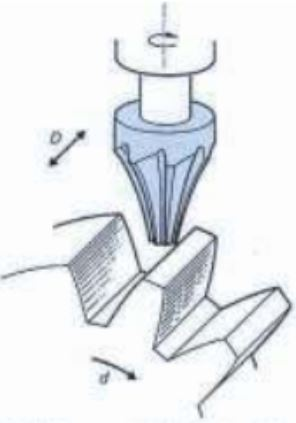
\includegraphics[width=0.5\linewidth]{Images/C1.JPG}
\end{minipage}
\begin{minipage}[t]{.44\linewidth}
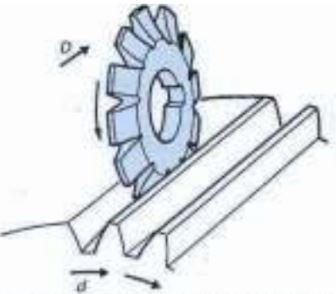
\includegraphics[width=0.7\linewidth]{Images/C2.JPG}
\end{minipage}


\begin{tcolorbox}[colback=blue!5!white,colframe=red!75!black]
  \bcinfo Les livres de production sont à votre disposition dans l'atelier
\end{tcolorbox}


\subsection{Tournage}
\begin{exo} Complétez le tableau d'opération d'usinage en tournage sur le document réponse. Vous devrez renseigner le ou les noms des opérations, la ou les formes/surfaces engendrées et enfin le ou les noms complets des outils.  \end{exo}

\subsection{Fraisage}
\begin{exo} Complétez le tableau d'opération d'usinage en fraisage sur le document réponse. Vous devrez renseigner le ou les noms des opérations, la ou les formes/surfaces engendrées et enfin le ou les noms complet des outils.  \end{exo}






\section{Désignation des outils}
\subsection{Introduction}


\begin{minipage}{.55\linewidth}
Au cours du BTS CPRP, vous devrez apprendre à choisir les bons outils et à savoir les monter sur une machine-outil. Vous devrez connaître les différents moyens d’attachements entre la machine, le porte outil et l’outil.
\end{minipage}
\begin{minipage}{.44\linewidth}
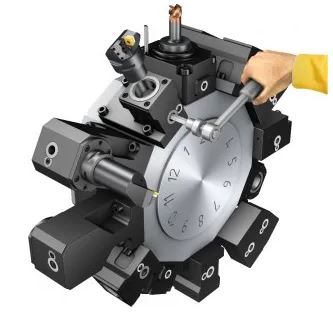
\includegraphics[width=0.7\linewidth]{Images/Outil2.JPG}
\end{minipage}



On s'intéressera en introduction à l'influence des technologie d'attachement comme "paramètre" à prendre en compte. Pourquoi avoir différentes façon d'attacher (de créer une liaison encastrement) les éléments aux autres, et quels impacts peut-on observer ? \\


\begin{minipage}{.55\linewidth}
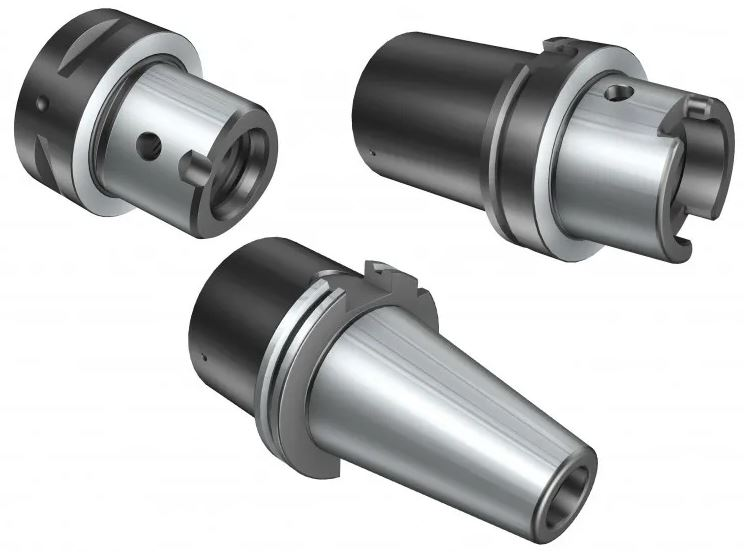
\includegraphics[width=0.7\linewidth]{Images/Outil3.JPG}
\end{minipage}
\begin{minipage}{.44\linewidth}
Vous avez sans doute remarqué qu'il existe plusieurs types d'attaches pour insérer les outils. Ceux-ci disposent de formes et de technologies d'attaches différentes. Pour réduire le temps d'usinage, il faut que l'interface de broche autorise des changements rapides d'outils. 
\end{minipage}

%%%%%%%%%%%%%%%%%%%%%%%%%%%%%%%%%%%%%%%%%%%%%%%%%%%%%%%%%%%%%%%%%%%%%%%%%%%%%%%%
%%%%%%%%%%%%%%%%%%%%%%%%%%%%%%%%%%%%%%%%%%%%%%%%%%%%%%%%%%%%%%%%%%%%%%%%%%%%%%%%

\begin{center}


\tikzset{every picture/.style={line width=0.75pt}} %set default line width to 0.75pt        

\begin{tikzpicture}[x=0.75pt,y=0.75pt,yscale=-1,xscale=1]
%uncomment if require: \path (0,269); %set diagram left start at 0, and has height of 269

%Shape: Cube [id:dp2857128060847711] 
\draw   (4.5,258) -- (70,192.5) -- (679.25,192.5) -- (679.25,197) -- (613.75,262.5) -- (4.5,262.5) -- cycle ; \draw   (679.25,192.5) -- (613.75,258) -- (4.5,258) ; \draw   (613.75,258) -- (613.75,262.5) ;
%Shape: Resistor [id:dp6305555130716705] 
\draw   (494.02,117.38) -- (502.16,119.85) -- (506.66,111.55) -- (504.89,130.35) -- (513.89,113.75) -- (512.13,132.55) -- (521.12,115.95) -- (519.36,134.75) -- (528.36,118.15) -- (526.59,136.95) -- (531.09,128.65) -- (539.23,131.12) ;
%Straight Lines [id:da4039015473125058] 
\draw    (539.23,131.12) -- (570.75,143.5) ;
%Straight Lines [id:da287466354488114] 
\draw    (472.75,97.5) -- (494.02,117.38) ;
%Shape: Speaker [id:dp0640612939395977] 
\draw  [fill={rgb, 255:red, 255; green, 255; blue, 255 }  ,fill opacity=1 ] (44.75,184.5) -- (44.75,244.5) -- (76.45,226.5) -- (92.3,226.5) -- (92.3,202.5) -- (76.45,202.5) -- (44.75,184.5) -- cycle (124,208.5) -- (92.3,208.5) (124,220.5) -- (92.3,220.5) (76.45,226.5) -- (76.45,202.5) ;
%Shape: Resistor [id:dp6433376777702962] 
\draw   (339.13,83.05) -- (344.08,83.73) -- (345.92,78.49) -- (346.64,89.56) -- (350.31,79.1) -- (351.04,90.16) -- (354.71,79.7) -- (355.44,90.77) -- (359.11,80.3) -- (359.83,91.37) -- (361.67,86.14) -- (366.62,86.82) ;
%Straight Lines [id:da6406807499272664] 
\draw    (366.62,86.82) -- (384.75,94.5) ;
%Straight Lines [id:da9075065743531485] 
\draw [color={rgb, 255:red, 245; green, 166; blue, 35 }  ,draw opacity=1 ] [dash pattern={on 4.5pt off 4.5pt}]  (316.75,82.75) -- (339.13,83.05) ;
%Shape: Resistor [id:dp7759438745707996] 
\draw  [color={rgb, 255:red, 245; green, 166; blue, 35 }  ,draw opacity=1 ] (234.13,120.97) -- (235.84,116.28) -- (231.11,113.38) -- (242.08,115) -- (232.63,109.21) -- (243.6,110.83) -- (234.15,105.03) -- (245.12,106.66) -- (235.67,100.86) -- (246.64,102.49) -- (241.91,99.59) -- (243.62,94.89) ;
%Straight Lines [id:da8310454650271508] 
\draw [color={rgb, 255:red, 245; green, 166; blue, 35 }  ,draw opacity=1 ] [dash pattern={on 4.5pt off 4.5pt}]  (246.25,86.5) -- (243.62,94.89) ;
%Straight Lines [id:da5447513728111515] 
\draw    (234.13,120.97) -- (231.25,125.5) ;
%Curve Lines [id:da5967960727982486] 
\draw [color={rgb, 255:red, 208; green, 2; blue, 27 }  ,draw opacity=1 ]   (379.25,202.5) .. controls (356.22,161.83) and (297.66,120.2) .. (252.03,111.96) ;
\draw [shift={(249.25,111.5)}, rotate = 8.65] [fill={rgb, 255:red, 208; green, 2; blue, 27 }  ,fill opacity=1 ][line width=0.08]  [draw opacity=0] (8.93,-4.29) -- (0,0) -- (8.93,4.29) -- cycle    ;
%Curve Lines [id:da5686686838763104] 
\draw [color={rgb, 255:red, 208; green, 2; blue, 27 }  ,draw opacity=1 ]   (379.25,202.5) .. controls (376.8,183.39) and (365.23,143.63) .. (354.41,97.34) ;
\draw [shift={(353.75,94.5)}, rotate = 76.96] [fill={rgb, 255:red, 208; green, 2; blue, 27 }  ,fill opacity=1 ][line width=0.08]  [draw opacity=0] (8.93,-4.29) -- (0,0) -- (8.93,4.29) -- cycle    ;
%Curve Lines [id:da08795824886908421] 
\draw [color={rgb, 255:red, 208; green, 2; blue, 27 }  ,draw opacity=1 ]   (379.25,202.5) .. controls (416.87,172.8) and (455.96,183.77) .. (507.19,140.82) ;
\draw [shift={(508.75,139.5)}, rotate = 139.44] [fill={rgb, 255:red, 208; green, 2; blue, 27 }  ,fill opacity=1 ][line width=0.08]  [draw opacity=0] (8.93,-4.29) -- (0,0) -- (8.93,4.29) -- cycle    ;
%Curve Lines [id:da5366294203423299] 
\draw [color={rgb, 255:red, 65; green, 117; blue, 5 }  ,draw opacity=1 ]   (258.25,32) .. controls (242.57,40.82) and (207.68,57.32) .. (227.94,98.92) ;
\draw [shift={(229.25,101.5)}, rotate = 242.13] [fill={rgb, 255:red, 65; green, 117; blue, 5 }  ,fill opacity=1 ][line width=0.08]  [draw opacity=0] (8.93,-4.29) -- (0,0) -- (8.93,4.29) -- cycle    ;
%Curve Lines [id:da9790292400460139] 
\draw [color={rgb, 255:red, 65; green, 117; blue, 5 }  ,draw opacity=1 ]   (258.25,32) .. controls (290.1,43.76) and (319.55,37.75) .. (351.77,72.33) ;
\draw [shift={(353.75,74.5)}, rotate = 228.27] [fill={rgb, 255:red, 65; green, 117; blue, 5 }  ,fill opacity=1 ][line width=0.08]  [draw opacity=0] (8.93,-4.29) -- (0,0) -- (8.93,4.29) -- cycle    ;
%Shape: Ellipse [id:dp4296755779480679] 
\draw   (197.25,134.75) .. controls (197.25,129.37) and (208.33,125) .. (222,125) .. controls (235.67,125) and (246.75,129.37) .. (246.75,134.75) .. controls (246.75,140.13) and (235.67,144.5) .. (222,144.5) .. controls (208.33,144.5) and (197.25,140.13) .. (197.25,134.75) -- cycle ;
%Shape: Ellipse [id:dp14047140906301792] 
\draw  [color={rgb, 255:red, 245; green, 166; blue, 35 }  ,draw opacity=1 ][dash pattern={on 4.5pt off 4.5pt}] (244.75,82.75) .. controls (244.75,75.43) and (260.87,69.5) .. (280.75,69.5) .. controls (300.63,69.5) and (316.75,75.43) .. (316.75,82.75) .. controls (316.75,90.07) and (300.63,96) .. (280.75,96) .. controls (260.87,96) and (244.75,90.07) .. (244.75,82.75) -- cycle ;
%Shape: Ellipse [id:dp4068194395007667] 
\draw   (383.25,97.5) .. controls (383.25,83.69) and (403.29,72.5) .. (428,72.5) .. controls (452.71,72.5) and (472.75,83.69) .. (472.75,97.5) .. controls (472.75,111.31) and (452.71,122.5) .. (428,122.5) .. controls (403.29,122.5) and (383.25,111.31) .. (383.25,97.5) -- cycle ;
%Shape: Ellipse [id:dp20614519807136356] 
\draw   (570.75,143.5) .. controls (570.75,137.7) and (581.83,133) .. (595.5,133) .. controls (609.17,133) and (620.25,137.7) .. (620.25,143.5) .. controls (620.25,149.3) and (609.17,154) .. (595.5,154) .. controls (581.83,154) and (570.75,149.3) .. (570.75,143.5) -- cycle ;
%Flowchart: Manual Operation [id:dp2516876734294693] 
\draw  [color={rgb, 255:red, 245; green, 166; blue, 35 }  ,draw opacity=1 ] (175.75,100.94) -- (127,106) -- (127,79) -- (175.75,84.06) -- cycle ;
%Shape: Can [id:dp47688228089586504] 
\draw  [color={rgb, 255:red, 245; green, 166; blue, 35 }  ,draw opacity=1 ] (123.27,89) -- (173.98,89) .. controls (174.82,89) and (175.5,90.57) .. (175.5,92.5) .. controls (175.5,94.43) and (174.82,96) .. (173.98,96) -- (123.27,96) .. controls (122.43,96) and (121.75,94.43) .. (121.75,92.5) .. controls (121.75,90.57) and (122.43,89) .. (123.27,89) .. controls (124.1,89) and (124.78,90.57) .. (124.78,92.5) .. controls (124.78,94.43) and (124.1,96) .. (123.27,96) ;

%Curve Lines [id:da6435590994672398] 
\draw [color={rgb, 255:red, 245; green, 166; blue, 35 }  ,draw opacity=1 ] [dash pattern={on 4.5pt off 4.5pt}]  (113.25,66.5) .. controls (109.77,110.78) and (117.18,124.36) .. (227.09,109.23) ;
\draw [shift={(228.75,109)}, rotate = 172.09] [fill={rgb, 255:red, 245; green, 166; blue, 35 }  ,fill opacity=1 ][line width=0.08]  [draw opacity=0] (8.93,-4.29) -- (0,0) -- (8.93,4.29) -- cycle    ;

% Text Node
\draw (595.5,143.5) node  [font=\scriptsize] [align=left] {Bâti};
% Text Node
\draw  [fill={rgb, 255:red, 255; green, 255; blue, 255 }  ,fill opacity=1 ]  (154.14, 213.6) circle [x radius= 31.11, y radius= 24.04]   ;
\draw (154.14,213.6) node  [font=\footnotesize] [align=left] {\begin{minipage}[lt]{29.94pt}\setlength\topsep{0pt}
\begin{center}
Pièce à\\usiner
\end{center}

\end{minipage}};
% Text Node
\draw (280.75,82.75) node  [font=\scriptsize] [align=left] {\begin{minipage}[lt]{36.85pt}\setlength\topsep{0pt}
\begin{center}
Porte-Outil
\end{center}

\end{minipage}};
% Text Node
\draw (222,134.75) node  [font=\scriptsize] [align=left] {\begin{minipage}[lt]{17.4pt}\setlength\topsep{0pt}
\begin{center}
Outil
\end{center}

\end{minipage}};
% Text Node
\draw  [color={rgb, 255:red, 208; green, 2; blue, 27 }  ,draw opacity=1 ][fill={rgb, 255:red, 255; green, 255; blue, 255 }  ,fill opacity=1 ]  (289.5,203.5) -- (469.5,203.5) -- (469.5,226.5) -- (289.5,226.5) -- cycle  ;
\draw (292.5,207.5) node [anchor=north west][inner sep=0.75pt]  [font=\small,color={rgb, 255:red, 208; green, 2; blue, 27 }  ,opacity=1 ] [align=left] {Liaison encastrement voulue};
% Text Node
\draw  [color={rgb, 255:red, 65; green, 117; blue, 5 }  ,draw opacity=1 ]  (172.5,10.5) -- (328.5,10.5) -- (328.5,29.5) -- (172.5,29.5) -- cycle  ;
\draw (175.5,14.5) node [anchor=north west][inner sep=0.75pt]  [font=\scriptsize,color={rgb, 255:red, 65; green, 117; blue, 5 }  ,opacity=1 ] [align=left] {Doit être démontable facilement};
% Text Node
\draw (428,97.5) node  [font=\scriptsize] [align=left] {\begin{minipage}[lt]{29.99pt}\setlength\topsep{0pt}
\begin{center}
{\footnotesize Magasin Porte-Outil}
\end{center}

\end{minipage}};
% Text Node
\draw  [color={rgb, 255:red, 245; green, 166; blue, 35 }  ,draw opacity=1 ][dash pattern={on 4.5pt off 4.5pt}]  (69,46.5) -- (163,46.5) -- (163,65.5) -- (69,65.5) -- cycle  ;
\draw (72,50.5) node [anchor=north west][inner sep=0.75pt]  [font=\scriptsize,color={rgb, 255:red, 245; green, 166; blue, 35 }  ,opacity=1 ] [align=left] {Système d'attache};


\end{tikzpicture}
\end{center}


%%%%%%%%%%%%%%%%%%%%%%%%%%%%%%%%%%%%%%%%%%%%%%%%%%%%%%%%%%%%%%%%%%%%%%%%%%%%%%%%
%%%%%%%%%%%%%%%%%%%%%%%%%%%%%%%%%%%%%%%%%%%%%%%%%%%%%%%%%%%%%%%%%%%%%%%%%%%%%%%%


\begin{exo} Quelles peuvent être les contraintes extérieures qui agissent sur le systèmes d'attache lors d'un usinage ? Vous citerez au moins 4 contraintes.\end{exo}

\begin{exo} Quelles doivent être les caractéristiques principales des broches d'attaches ? Vous citerez au moins 3 caractéristiques.\end{exo}



L'université RWTH d'Aix-la-Chapelle (Allemagne) a mené une série de tests statiques dans le laboratoire machines-outils (WZL) pour comparer la résistance à la flexion et la transmission du couple de différentes interfaces d'attache de broches. Les résultats se présentent Figure \ref{T11}.

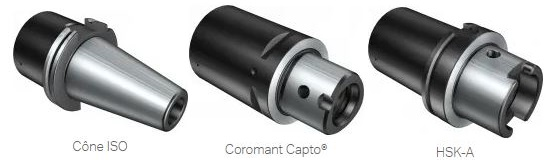
\includegraphics[width=0.9\linewidth]{Images/cone1.JPG}


\begin{exo} A l’aide du graphique figure \ref{T11}, \textbf{justifiez} quelle est l’attache avec la meilleure transmission du couple pour les essais effectués. \end{exo}

\subsection{Les outils en tournage}


\begin{tcolorbox}[colback=blue!5!white,colframe=red!75!black]
  \bcinfo Les livres de production sont à votre disposition dans l'atelier
\end{tcolorbox}

\begin{exo} Nommez les différents éléments de l’outil d’usinage figure \ref{PP1} à l'aide des mots
indiques dans le dossier réponse. \end{exo}

\begin{minipage}{.55\linewidth}
\begin{itemize}
    \item Porte-outil;
    \item Sortie huile de coupe
    \item Liaison vis sans fin
\end{itemize} 
\end{minipage}
\begin{minipage}{.44\linewidth}
\begin{itemize}
    \item Plaquettes
    \item Cales
    \item Porte plaquette
\end{itemize} 
\end{minipage}




\subsection{Les outils en fraisage}


\begin{exo} Nommez les différents éléments de l’outil d’usinage figure \ref{FF1} à l'aide des mots
indiques dans le dossier réponse. \end{exo}



\begin{minipage}{.55\linewidth}
\begin{itemize}
    \item Porte-outil;
    \item Foret monobloc
    \item Liaison vis sans fin
    \item Clavette d'entraînement (transmission du couple)
\end{itemize} 
\end{minipage}
\begin{minipage}{.44\linewidth}
\begin{itemize}
    \item Outil
    \item Dispositif de serrage
    \item Magasin outil / Tourelle
\end{itemize} 
\end{minipage}


\section{Sélection des plaquettes - Application}
Les fabricants d’outils mettent à notre disposition une multitude de plaquettes et de porte-plaquettes différents. En temps que technicien d’usinage, nous serons amenés à reconnaître et aussi à choisir le type d’outil le plus adapté à une opération d’usinage donnée afin de commander chez le fabricant l’outil idéal.


\subsection{Fabrication des plaquettes d'usinages}
La plupart des plaquettes carbure que vous verrez s'inscrit dans un processus défini avec soin visant à produire un équilibre entre la géométrie et la nuance afin d'obtenir un produit parfaitement adapté à l'application.

\begin{center}
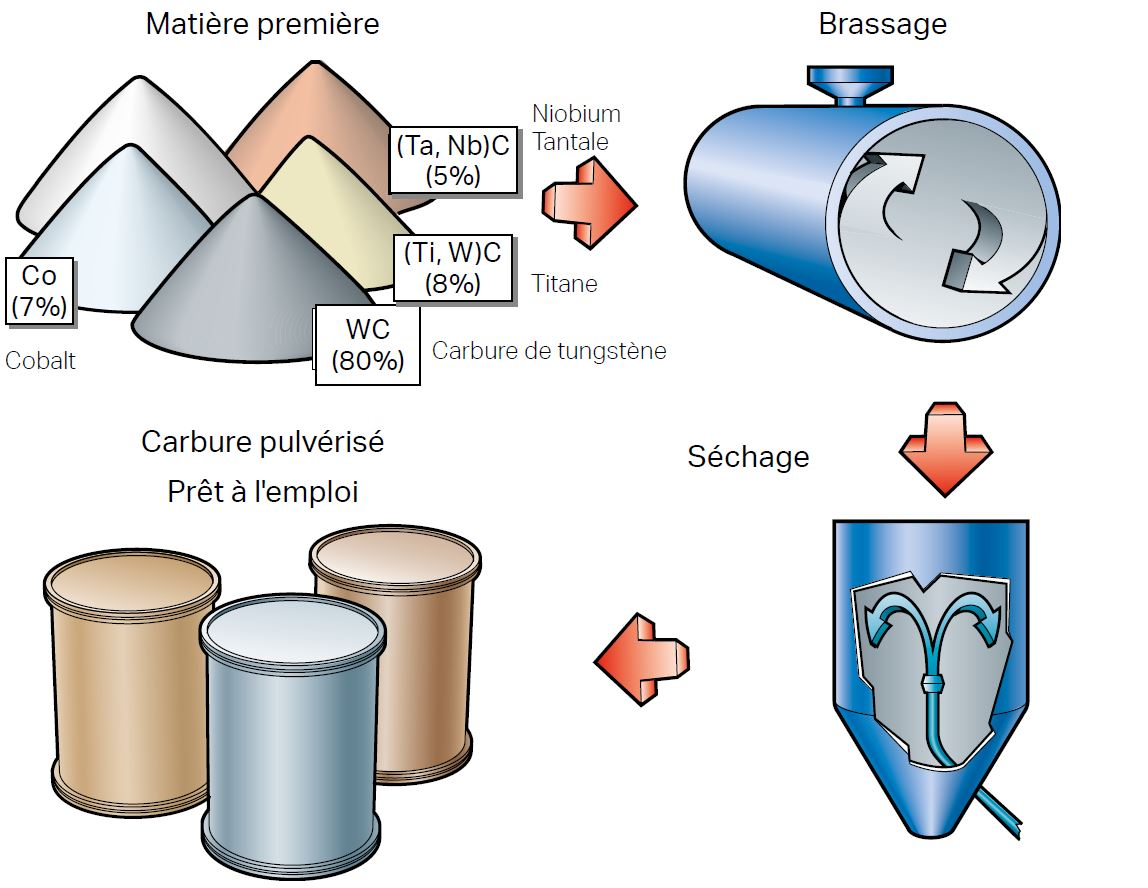
\includegraphics[width=0.7\linewidth]{Images/PLA11.JPG}
\end{center}

Au début la matière première est constituée de sable de carbure de tungstène, de sable de Cobalt et d'autres éléments. Ce sable de matière est appelé \textbf{poudre}. La poudre passe ensuite une étape qui lui donne la forme d'une plaquette.



\begin{center}
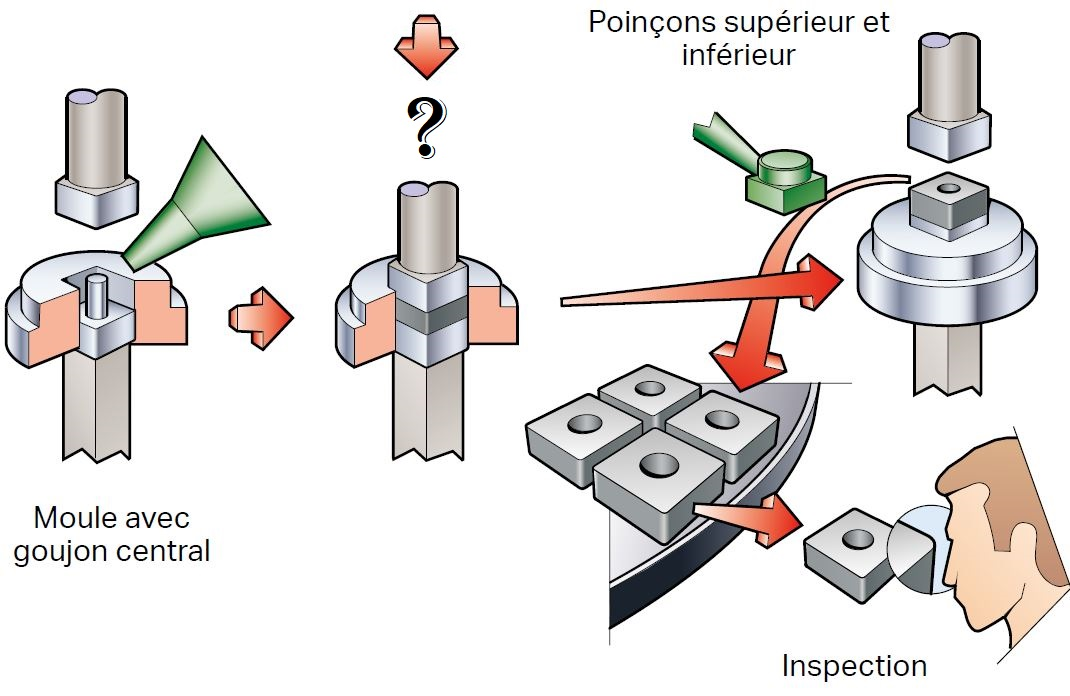
\includegraphics[width=0.7\linewidth]{Images/PLA12.JPG}
\end{center}

\begin{exo} Quel est le type de procédé utilisé pour lié le mélange de poudre dans le processus de fabrication des plaquettes ?\end{exo}

\noindent
La plaquette passe ensuite par un procédé de frittage.


\begin{center}
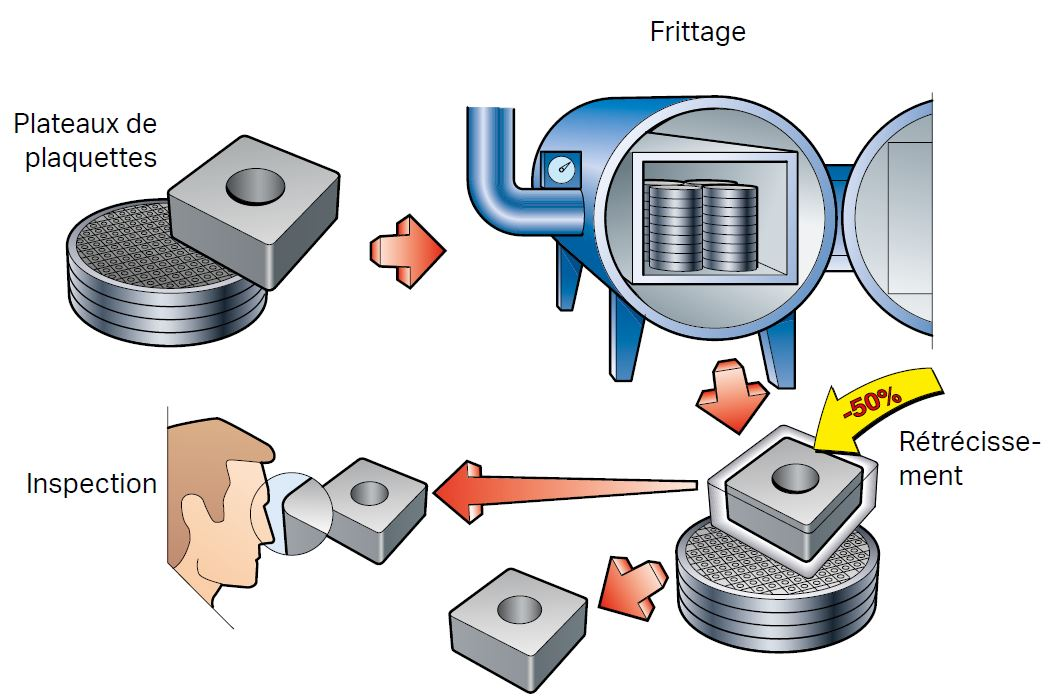
\includegraphics[width=0.7\linewidth]{Images/PLA13.JPG}
\end{center}


\begin{exo} Expliquez en quoi consiste un procédé de \textbf{frittage}.\end{exo}


\begin{minipage}{.55\linewidth}
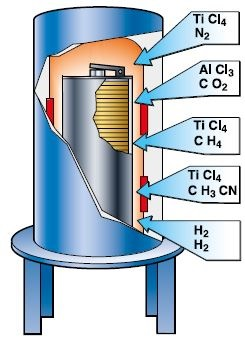
\includegraphics[width=0.7\linewidth]{Images/PLA15.JPG}
\end{minipage}
\begin{minipage}{.44\linewidth}
La plaquette effectuera ensuite plusieurs sortes d'opérations de rectification, un traitement très précis qui donnera sa micro-géométrie finale à l'arête de coupe, et enfin les plaquettes sont empilées et placées dans un four. Des séries de gaz sont successivement introduites dans l'enceinte en alternance avec du vide. Ces opérations créent les différentes couches du revêtement. Le processus est effectué à une température d'environ 900°C et prend une trentaine d'heures. L'épaisseur est d'environ 2 à 20 microns.
\end{minipage}


\subsection{Partie active des outils coupant}

\begin{tcolorbox}[colback=blue!5!white,colframe=red!75!black]
  \bcinfo Les livres de production sont à votre disposition dans l'atelier
\end{tcolorbox}

\begin{exo} Trouvez le noms des différents éléments qui constituent la zone de coupe des outils en vous aidant des mots indiqués.\end{exo}
\begin{center}
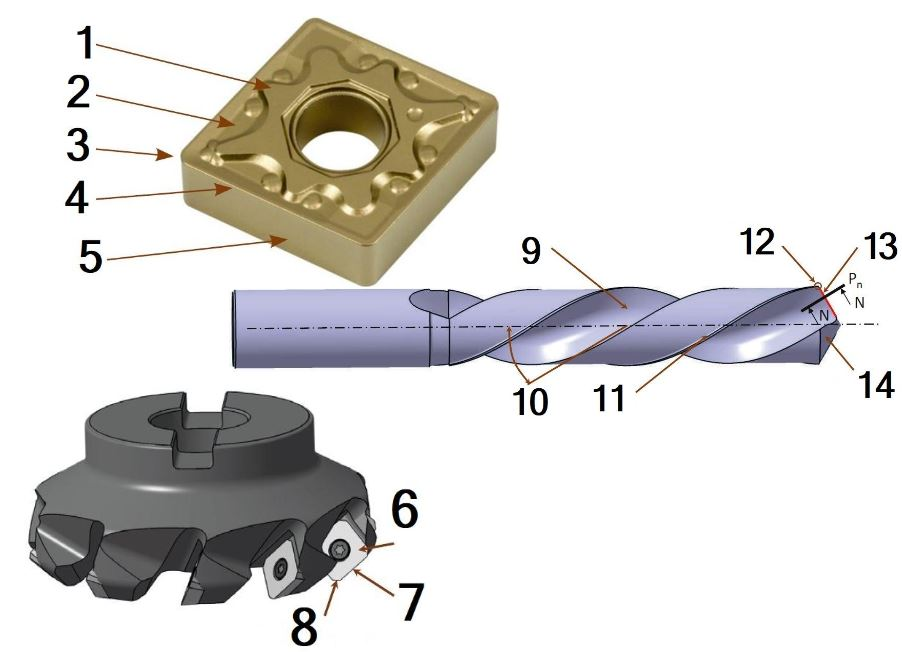
\includegraphics[width=1\linewidth]{Images/PLA20.JPG}
\end{center}





\section{Lubrification}
\begin{figure}[h]
\centering
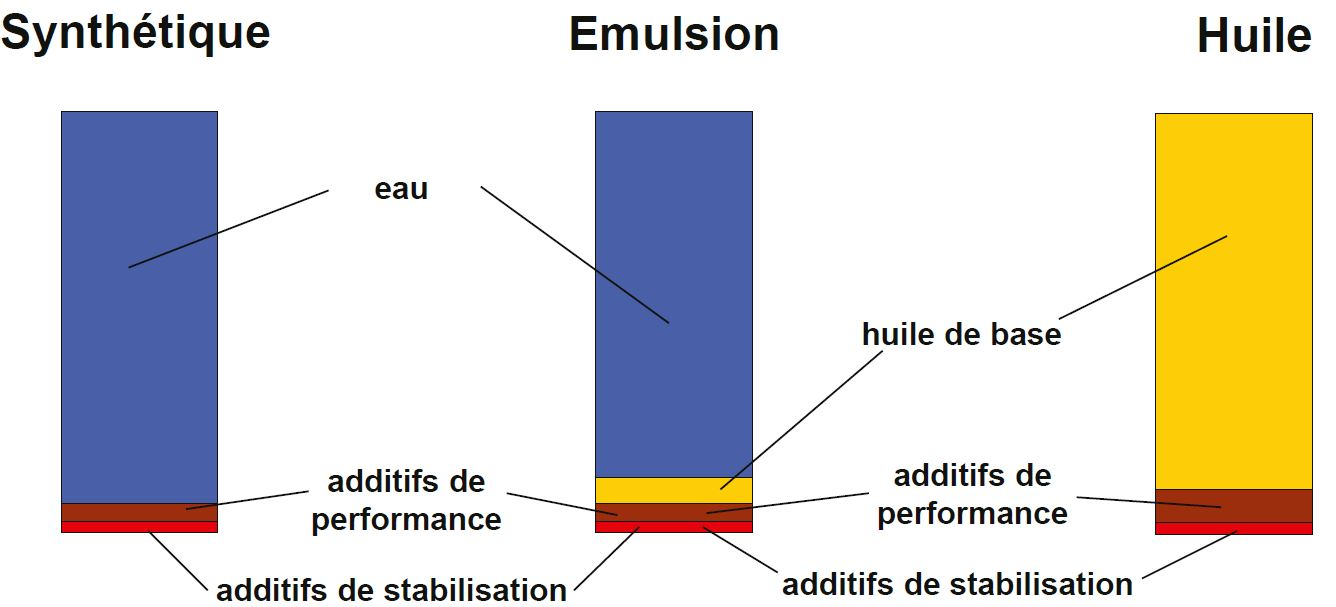
\includegraphics[width=0.7\linewidth]{Images/LU1.JPG}
\caption{Les principaux types de lubrifiants employés en usinage (Blaser).}
\label{bridppe}
\end{figure}

Dans certaines situations, les contraintes environnementales et les coûts peuvent rendre l'usinage à sec, sans liquide de coupe, préférable. Cependant de nombreuses applications nécessitent un arrosage pour obtenir de bonnes tolérances et une bonne qualité d'état de surface et pour favoriser l'usinabilité. L'arrosage, qu'il soit synthétique, une émulsion\footnote{Une émulsion est un mélange hétérogène de deux substances liquides non miscibles, l'une étant dispersée sous forme de petites gouttelettes dans l'autre. Ce sont toujours deux liquides qui ne se mélangent pas spontanément (non miscibles), comme l’eau et l’huile, mais qui vont grâce à des opérations spécifiques (agitation, mélange, ajout de quelques principes actifs) adopter un aspect macroscopiquement homogène, mais microscopiquement hétérogène.} ou de l'huile, doit être \textbf{optimisé} pour avoir une \textbf{efficacité} maximum. On compare ici deux technologies de lubrifications, internes et externes comme le montre les figures \ref{M1} et \ref{L13}.


\begin{exo} Quels peuvent être les deux intérêts principaux de l'utilisation d'une lubrification interne ou externe ? Comparez les deux technologies.\end{exo}


%%%%%%%%%%%%%%%%%%%%%%%%%%%%%%%%%%%%%%%%%%%%%%%%%%%%%%%%%%%%%%%%%%%%%%%%%%%%%%%%%%%%%%
%%%%%%%%%%%%%%%%%%%%%%%%%%%%%%%%%%%%%%%%%%%%%%%%%%%%%%%%%%%%%%%%%%%%%%%%%%%%%%%%%%%%%%
%%%%%%%%%%%%%%%%%%%%%%%%%%%%%%%%%%%%%%%%%%%%%%%%%%%%%%%%%%%%%%%%%%%%%%%%%%%%%%%%%%%%%%

\begin{tcolorbox}[colback=blue!5!white,colframe=red!75!black]
  \bcinfo szldkjfvhspdjfnmzekjfnmlsqdkjfnmlskdjfnlksmqdjf
\end{tcolorbox}


\section{ANNEXE}
\begin{tcolorbox}[colback=blue!5!white,colframe=orange!75!black]
\begin{center}
    \textbf{Glossaire :}
\end{center}
\begin{itemize}
    \item CNC : Computer Numerical Control (Commande numérique par calculateur);
    \item MOCN : Machine Outil à commande numérique, elle est programmable et équipée d'une "commande numérique par calculateur" (CNC). Elle est en général dédiée à des fabrication variées de pièces différentes, lancées en petits lots répétitifs.
    \item CU : Centre d'usinage : En fait, c'est une MOCN qui est complétée d'autres équipement périphériques qui assurent notamment : \begin{itemize}
        \item le changement automatique d'outils stockés dans des magasins d'outils;
        \item le changement automatique de pièce (palettisation)
        \item éventuellement le convoyage des copeaux (convoyeur)
    \end{itemize}
    Il est dédié à des fabrications variées de pièces différentes.
    \item CAO : Conception Assistée par Ordinateur;
    \item FAO : Fabrication Assistée par Ordinateur;
    \item MQL : Minimum Quantity Lubrication .
\end{itemize}
\end{tcolorbox}


\begin{figure}
\centering
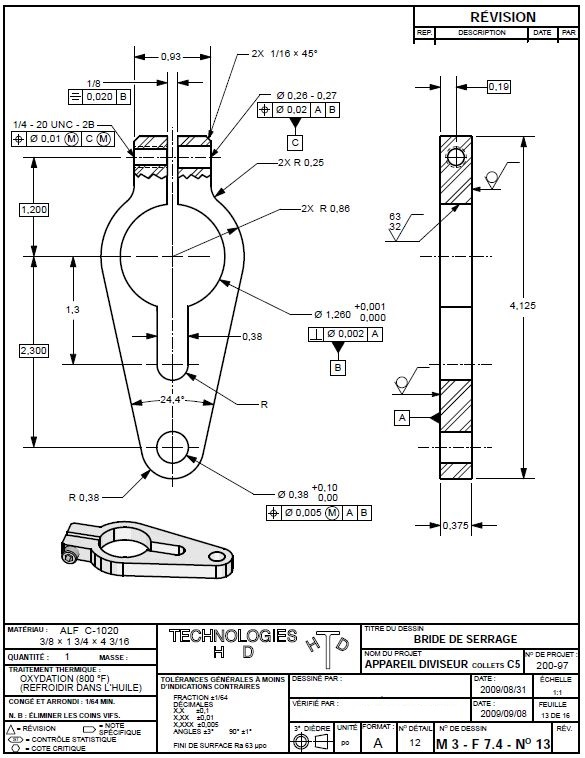
\includegraphics[width=0.9\linewidth]{Images/dessin1.JPG}
\caption{Dessin de définition d'une bride de serrage}
\label{bride}
\end{figure}




\begin{figure}
\centering
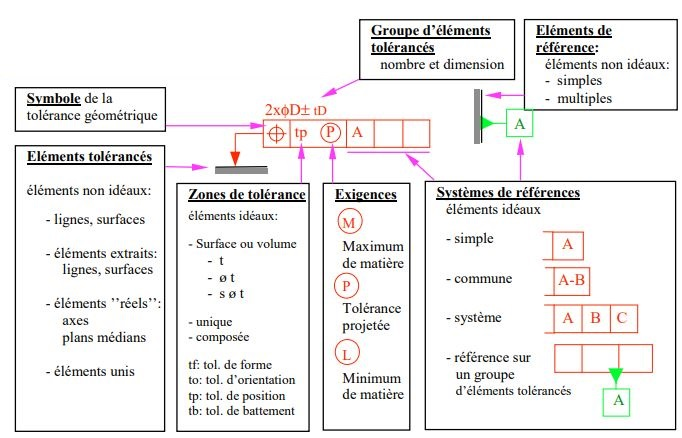
\includegraphics[width=0.9\linewidth]{Images/gps.JPG}
\caption{Aide mémoire pour spécification géométrique}
\label{gps}
\end{figure}


\begin{figure}
\centering
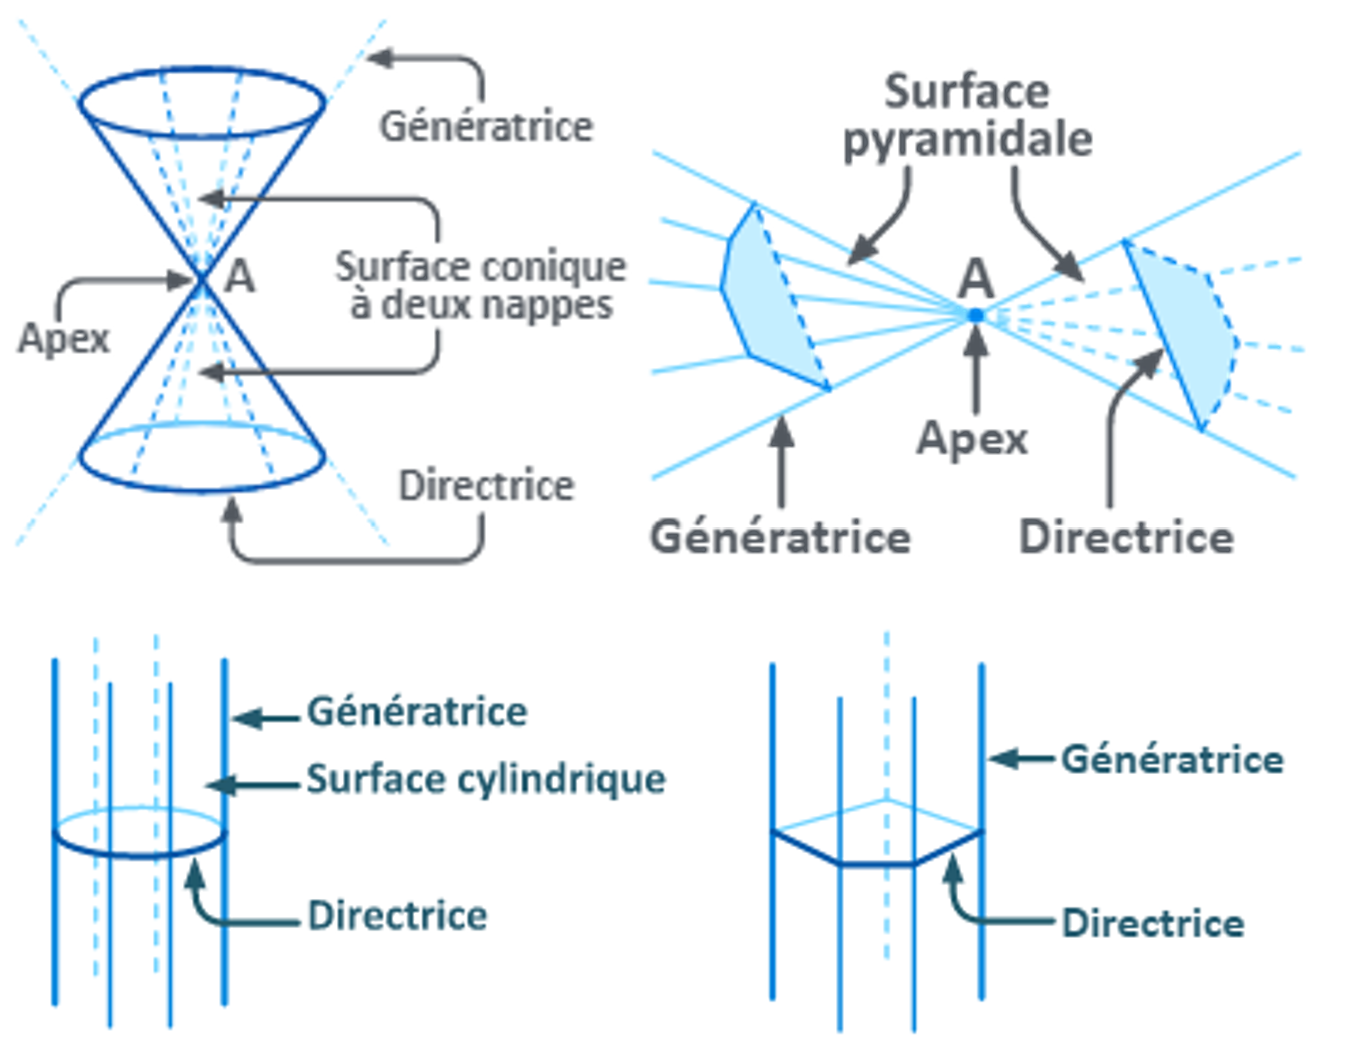
\includegraphics[width=0.9\linewidth]{Images/directrice.png}
\caption{Directrice : Ligne simple fermée sur laquelle s’appuie une droite mobile, appelée génératrice, en engendrant une surface. La génératrice engendre une surface conique, si cette directrice est une ligne courbe fermée (dessin en bas à gauche), ou bien, engendre une surface pyramidale, si cette directrice est un polygone (dessin en bas à droite).}
\label{directrice}
\end{figure}


\begin{figure}
\centering
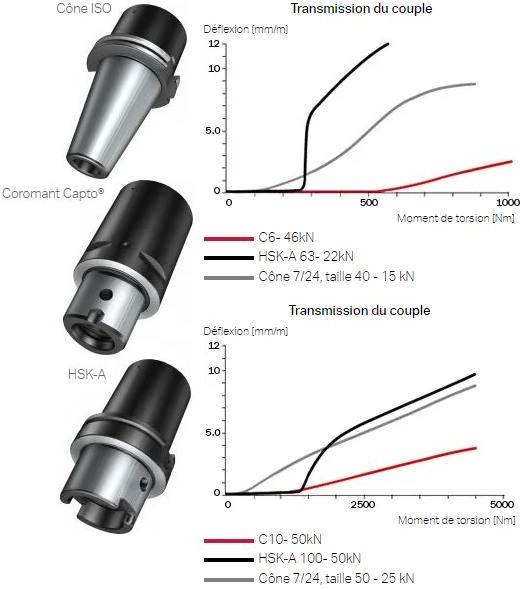
\includegraphics[width=0.8\linewidth]{Images/T11.JPG}
\caption{Tests statiques pour comparer la résistance à la flexion et la transmission du couple de différentes interfaces de broches. Coromant Capto a été testé avec deux forces de serrage : la force de serrage de HSK-A, (22 kN pour C6 et 50 kN pour C10) et la force de serrage maximum standard (45 kN pour C6 et 80 kN pour C10).}
\label{T11}
\end{figure}


\begin{figure}
\centering
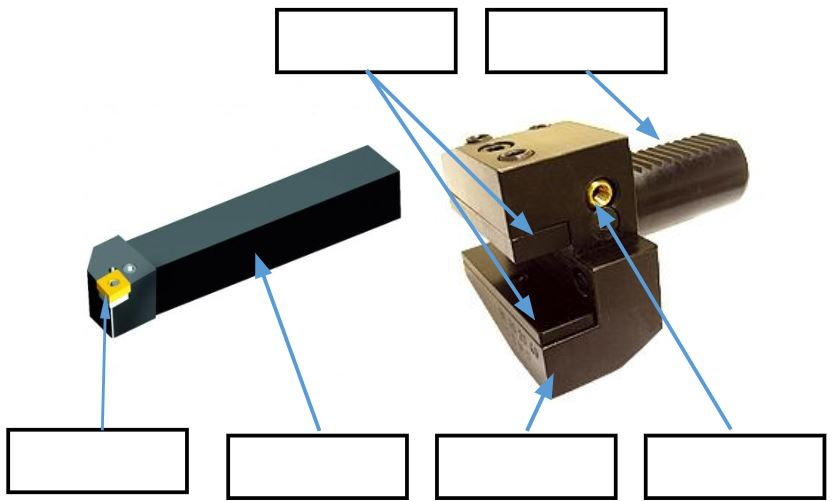
\includegraphics[width=0.8\linewidth]{Images/PP1.JPG}
\caption{RÉPONDRE SUR DOSSIER RÉPONSE.}
\label{PP1}
\end{figure}


\begin{figure}
\centering
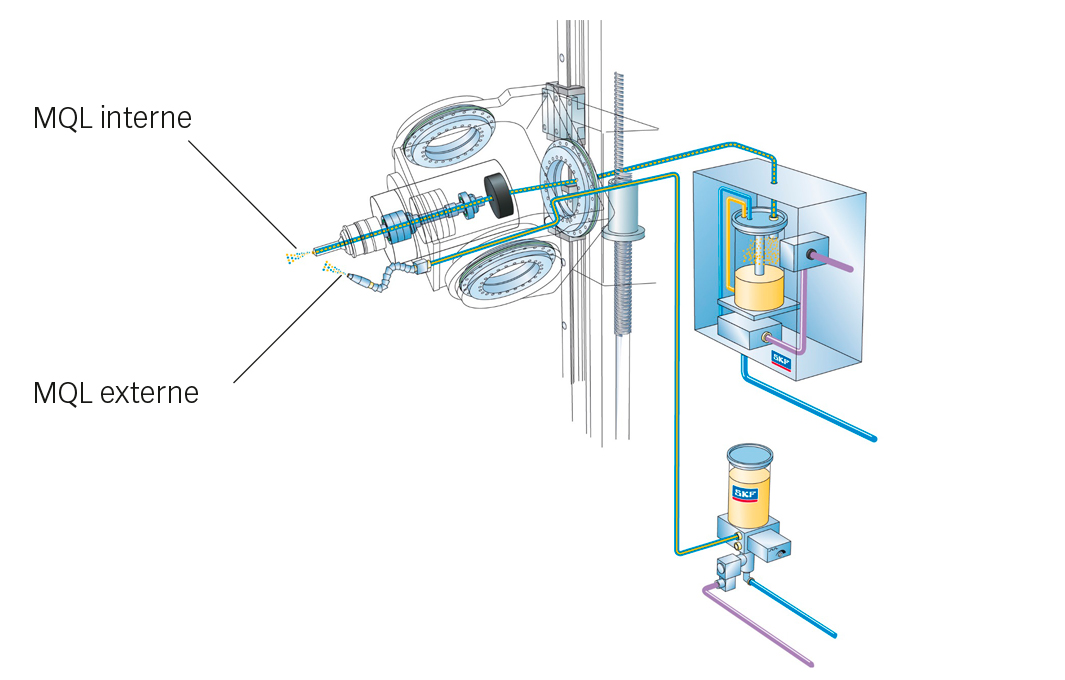
\includegraphics[width=0.9\linewidth]{Images/M1.jpg}
\caption{Microlubrification MQL interne et externe de SKF}
\label{M1}
\end{figure}



\begin{figure}
\centering
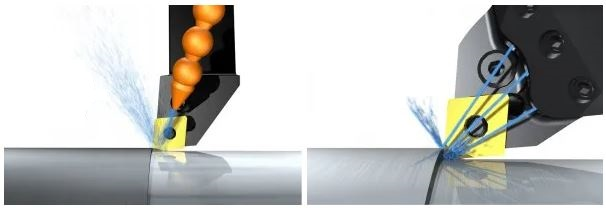
\includegraphics[width=0.9\linewidth]{Images/L13.jpg}
\caption{Dispositif de lubrification externe - à gauche, et lubrification interne - à droite.}
\label{L13}
\end{figure}



\begin{figure}
\centering
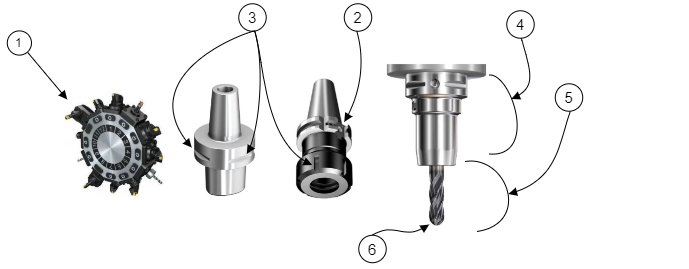
\includegraphics[width=1\linewidth]{Images/FF1.png}
\caption{Éléments de centre d'usinage. RÉPONDRE SUR DOSSIER RÉPONSE.}
\label{FF1}
\end{figure}



\end{document}

